\documentclass[00_doc.tex]{subfiles}
\begin{document}
    \subsection{Merging Code and Physical Components}
    \begin{flushleft}
        After coding everything and testing the code if everything is working as we plant, we glued
        the blossom and the base together. Furthermore, we added a plastic half ball, on top of the 
        RGB-LEDs (see Figure ~\ref{fig:finalPrototyp}).
    \end{flushleft}

    \begin{table}[h!]
        \centering
        \begin{tabular}{c}
        \centering
        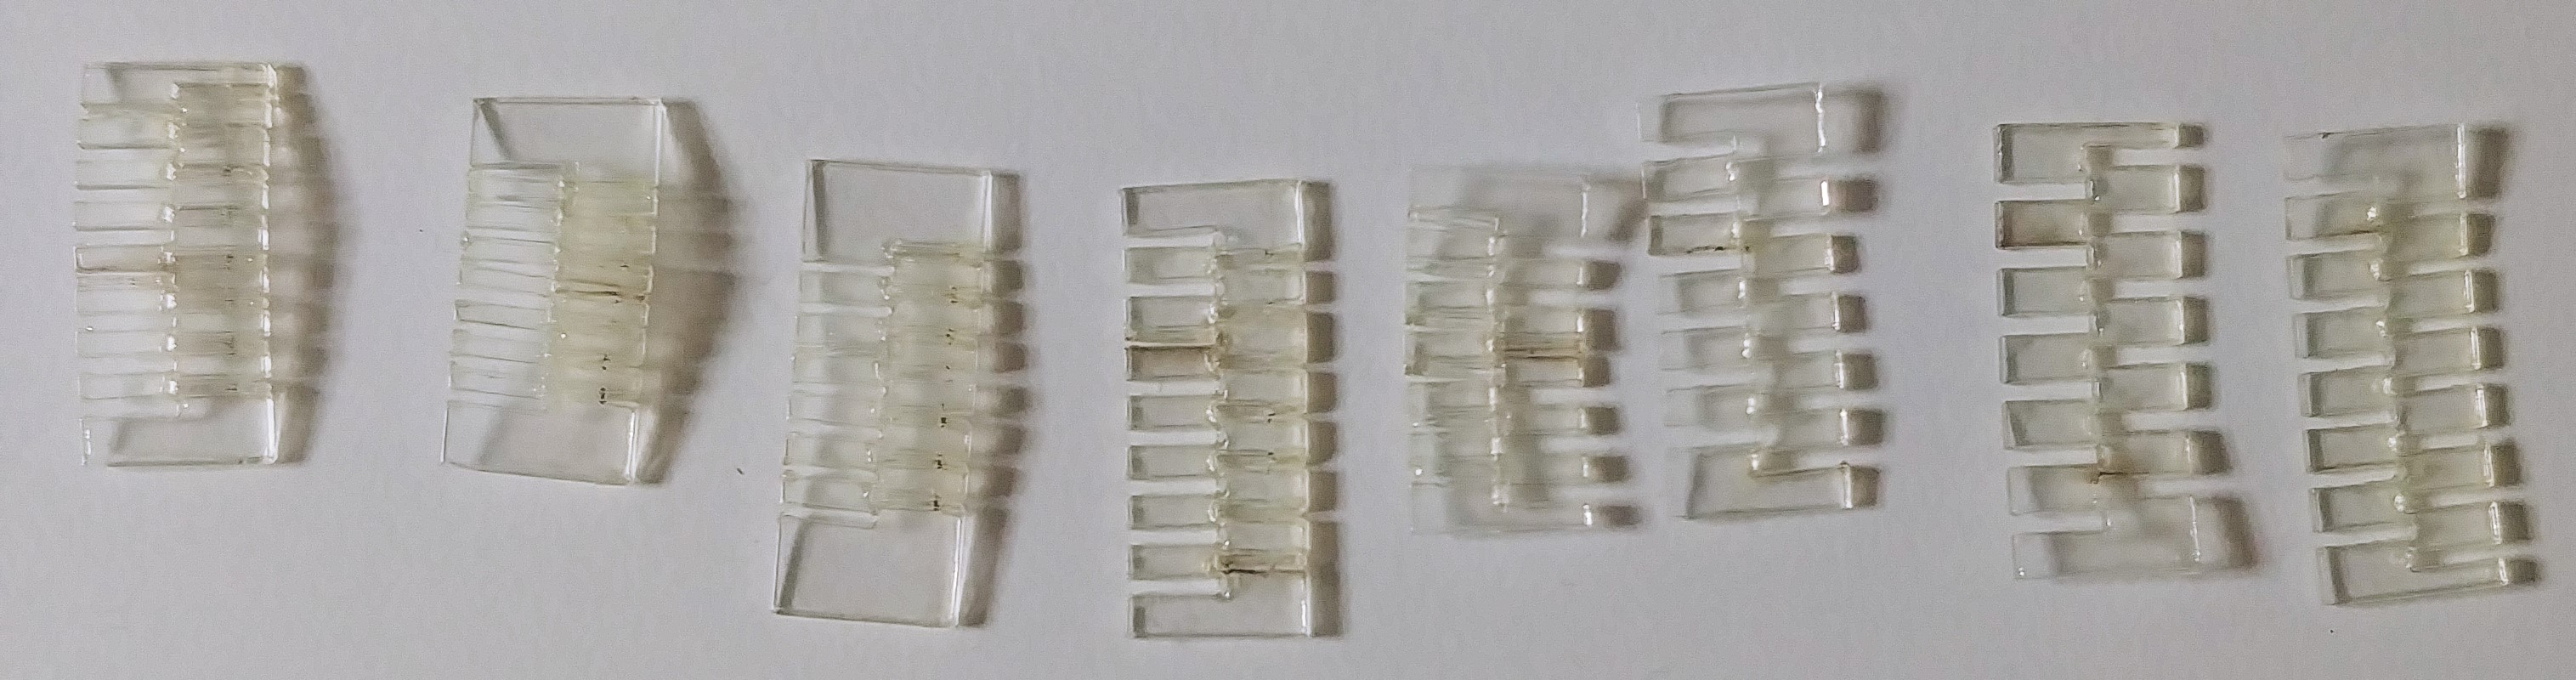
\includegraphics[width=.8\linewidth]{images/process/01_LaserCut.jpg}
        \end{tabular}
        \caption{Shows the final prototyp of the blossom shaped lamp.}
        \label{fig:finalPrototyp}
    \end{table}
\end{document}
